\documentclass[leqno]{article}
\author{Colin Roberts}
\usepackage{preamble}

\begin{document}

\begin{center}
  \begin{huge}
    MATH 666: Advanced Algebra I
  \end{huge}
\end{center}

\section*{Homework assignment 4 -- due 9/27/2019}
\noindent \emph{I worked with Brittany and Brenden.}
\setcounter{problem}{15}
\begin{problem}
Let $p$ be prime and $G=\SL_2(\finitef_p)$, acting on the space $V_m$ of
homogeneous polynomials of degree $m-1$ in $\finitef_p[x,y]$. Let $\delta$ be the
associated representation with respect to the basis
\[
(x^{m-1},x^{m-2}y,\cdots xy^{m-2},y^{m-1}).
\]
\begin{enumerate}[(a)]
    \item Describe $\delta(a)$,$\delta(b)$ for the two generators
\[
a=
\left(\begin{array}{cc}
1&1\\0&1
\end{array}
\right),\qquad
b=
\left(\begin{array}{cc}
1&0\\1&1
\end{array}
\right).
\]
\item Use {\sc Norton}'s irreducibility criterion for $a-1$ to show that $V_m$
is simple for $m\le p$.
\end{enumerate}
\end{problem}
\begin{solution}~
\begin{enumerate}[(a)]
    \item Consider 
    \begin{align*}
        (x^i y^j).a &= (x+y)^i y^j = y^j \sum_{k=0}^i \binom{i}{k}x^k y^{i-k}\\
        (x^i y^j).b &= x^i (x+y)^j = x^i \sum_{k=0}^j \binom{j}{k}x^k y^{i-k}.
    \end{align*}
    Notice that we get binomial coefficients, which allow us to arrange $\delta(a)$ and $\delta(b)$ as 
    \begin{align*}
        \delta(a)=\begin{pmatrix} \binom{m-1}{0} & \binom{m-1}{1} & \binom{m-1}{2} & \cdots & \binom{m-1}{m-1}\\ 
        \binom{m-2}{0} & \binom{m-2}{1} & \binom{m-2}{2} & \cdots & 0 \\
        \vdots & \vdots & \vdots & \ddots & \vdots \\
        1 & 0 & 0 & 0 & 0\end{pmatrix} \qquad \textrm{and} \qquad \delta(b)=\begin{pmatrix}          1 & 0 & 0 & 0 & 0\\
        \vdots & \vdots & \vdots & \ddots & \vdots \\
    \binom{m-2}{0} & \binom{m-2}{1} & \binom{m-2}{2} & \cdots & 0 \\
        \binom{m-1}{0} & \binom{m-1}{1} & \binom{m-1}{2} & \cdots & \binom{m-1}{m-1}\end{pmatrix}
    \end{align*}
    \item First, note that we have
    \[
    \delta(a-1) = \begin{pmatrix} 0 & 0 & 0 & \cdots & 1\\ 0 & 0 & 0 &\cdots & 1 \\ \vdots & \vdots & \vdots & \ddots & 1\end{pmatrix}
    \]
    so $\ker (\delta(a-1))\neq \{0\}$.  Note that there does not exist $v\in \ker (\delta(a-1))$ such that $\langle v \rangle_{\finitef_p G}$ forms a proper submodule as any vector 
    \[
    v = \alpha_{m-1}x^{m-1} + \alpha_{m-2}x^{m-2}y + \cdots + \alpha_{0}y^{m-1}
    \]
    will be mapped to 
    \[
    \delta(a-i)v = \left(\sum_{i=1}^{m-1}\alpha_{i}\right) y^{m-1}.
    \]
    A similar argument can be made for $w\in \ker (\delta^*(a-1))$ as this is just the transpose of the matrix $\delta(a-1)$ (or action from the left on column vectors).  Hence, we are left with $V_{m-1}$ is irreducible.
\end{enumerate}
\end{solution}

\newpage
\begin{problem}
Consider the group algebra $A=\finitef_2S_3$ for $S_3$ over the field with 2
elements.\\
a) Determine the submodules of $A_A$. (Hint: the {\sf GAP} commands {\tt
RegularModule(G,GF(2))[2];} and {\tt MTX.BasesSubmodules}.)\\
b) Determine the isomorphism types of simple modules ({\tt
MTX.CollectedFactors}).\\
c) Draw the submodule lattice for $A_A$ and identify the different $H^S(A)$
and $J(A)$. Hint: If {\tt b} is a list of submodule bases the following
{\sf GAP} commands below determine for each submodule those that it is included
in, and those in which it is a maximal submodule.
\end{problem}
\begin{solution}
See the included \textsf{GAP} code.
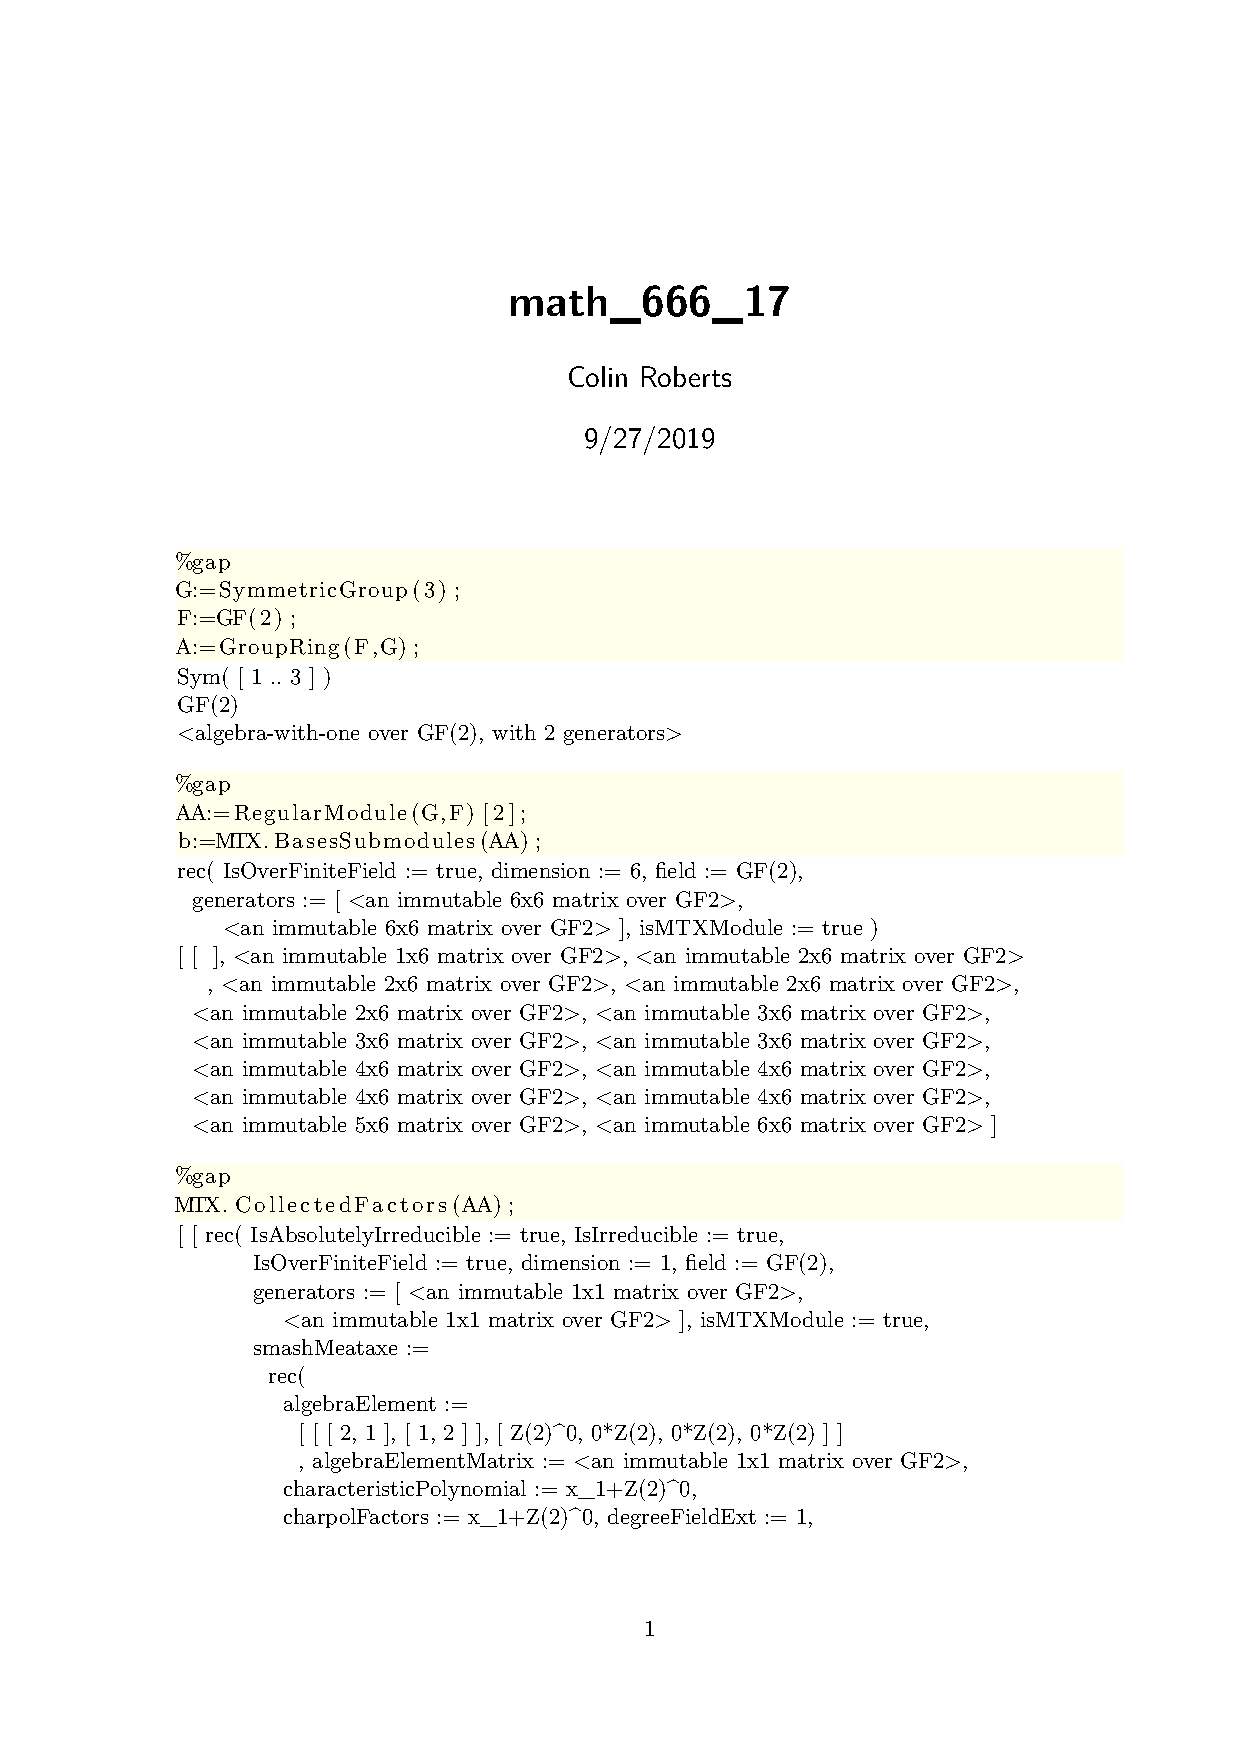
\includepdf[pages=-,pagecommand={},width=\textwidth]{Homework_4/math_666_17.pdf}
\end{solution}


\newpage
\begin{problem}
(Isomorphism test for irreducible modules)
Let $G=\left\langle g_1,\ldots,g_k\right\rangle$ a finite group,
$F$ be a field and
$\varphi,\psi\colon G\to\GL_n(F)$ be two equivalent irreducible
representations of a finite group $G$ (i.e.  there exists a matrix
$M\in\GL_n(F)$ such that for all $g\in G$: $M^{-1}(g^\varphi)M=g^\psi$.\\
The aim of this problem is to show a method to test constructively
for such an isomorphism.
\begin{enumerate}[(a)]
    \item Let $\omega\in FG$ be an element such that the nullity of $\omega^\varphi$
(i.e. the dimension of $\ker\omega^\varphi$)
is 1. Show that the nullity of $\omega^\psi$ is also 1.
\item Let $\mathbf{x}\in\ker(\omega^\varphi)$ and $\mathbf{y}\in\ker(\omega^\psi)$.
Show that there exists $\alpha\in F$ such that $\mathbf{x}\cdot
M=\alpha\cdot\mathbf{y}$.
\item We now start a spinning algorithm for 
$(g_1^\varphi,\ldots,g_k^\varphi)$, starting with $\mathbf{x}$, obtaining (as
$\varphi$ is irreducible) a basis
$\Bb=(\mathbf{x}_1:=\mathbf{x},\mathbf{x}_2,\ldots,\mathbf{x}_n)$ of $F^n$.

We also start (in parallel) 
a spinning algorithm for 
$(g_1^\psi,\ldots,g_k^\psi)$, starting with $\mathbf{y}$ and obtain a second
basis $\Cb=(\mathbf{y}_1:=\mathbf{y},\mathbf{y}_2,\ldots,\mathbf{y}_n)$ of $F^n$.

Show that:
\begin{enumerate}[1.]
\item $\mathbf{x}_i\cdot M=\alpha\cdot\mathbf{y}_i$, where $\alpha$ is as
defined in b).
\item For all $i,j,l$ we have that 
$\mathbf{x}_i\cdot g_j^\varphi\in\Span(\mathbf{x}_1,\ldots,\mathbf{x}_l)
\Leftrightarrow
\mathbf{y}_i\cdot g_j^\psi\in\Span(\mathbf{y}_1,\ldots,\mathbf{y}_l)$
\end{enumerate}
({\bf Hint:} It might be easiest to prove both statements together in one
induction. The second statement will be needed to show that both spinning
algorithms will define new elements $\mathbf{x}_i$ at exactly the same time in
the ``same'' way, which then proves the first statement.)\\
\item Let $N=\matbas{\Bb}{id}{\Cb}$ the matrix for base change from
(we act on the right) $\Bb$ to $\Cb$. Show that $N^{-1}a^\varphi N=a^\psi$,
i.e. that $N$ can serve as base change showing the equivalence of $\varphi$
and $\psi$.\medskip

{\bf Remark:} If the representations are not equivalent, either $\omega^\varphi$ and
$\omega^\psi$ will have different nullity, or the matrix
$\matbas{\Bb}{id}{\Cb}$ will not map $a^\varphi$ to $a^\psi$. This
methods thus gives a constructive isomorphism test for irreducible modules.
The command {\tt MTX.Isomorphism} in {\GAP} does exactly this test.
\end{enumerate}
\end{problem}
\begin{solution}~
\begin{enumerate}[(a)]
    \item Note that we have
    \[
    \omega^\psi = M^{-1} \omega^\varphi M.
    \]
    Now, since $M\in \GL_n(F)$, we have that $\nullity(M)=\nullity(M^{-1})=0$.  Hence, by composition, $\nullity(M^{-1} \omega^\varphi M)=1$ and so $\nullity(\omega^\psi)=1$.
    \item Take $x\in \ker \omega^\varphi$ and note that we have
    \begin{align*}
        \omega^\psi &= M^{-1} \omega^\varphi M\\
        \iff ~ M\omega^\psi &= \omega^\varphi M\\
        \iff ~ 0=\mathbf{x}M\omega^\psi &= \mathbf{x} \omega^\varphi M
    \end{align*}
    since $\mathbf{x}\in \ker \omega^\varphi$.  Hence, it follows that $\mathbf{x}M\in \ker \omega^\psi$ and since $\nullity(\omega^\psi)=1$, it must be that $\mathbf{x}M=\alpha \mathbf{y}$ for some $\alpha \in F$.
    \item We have the base case that for $\mathbf{x}_1 \in \ker \omega^\varphi$ we have $\mathbf{x}_1 M = \alpha \mathbf{y}_1$ from (b).  So now, assume this holds for vectors $\{\mathbf{x}_1,\mathbf{x}_2,\dots,\mathbf{x}_k\}$ and $\{\mathbf{y}_1,\mathbf{y}_2,\dots,\mathbf{y}_k\}$. 
    
    Then, take $x_i \omega_j^\varphi \in \Span\{\mathbf{x}_1,\dots,\mathbf{x}_{k+1}\}$. Then we can put 
    \begin{align*}
        \mathbf{x}_i \omega_j^\varphi &= \sum_{n=1}^{k+1} a_n \mathbf{x}_n\\
        \iff~ \mathbf{x}_i \omega_j^\varphi M &= \sum_{n=1}^{k} a_n \mathbf{x}_nM + a_{k+1}\mathbf{x}_{k+1}M.
    \end{align*}
    Now, note that we can write $\mathbf{x}_i\omega_j^\varphi M=\alpha \mathbf{y}_i M^{-1}\omega_j^\varphi M = \alpha \mathbf{y}_i \omega_j^\psi$.  Thus we have 
    \[
    \alpha \mathbf{y}_i \omega_j^\psi = \alpha \sum_{n=1}^k a_k \mathbf{y}_k + a_{k+1} \mathbf{x}_{k+1} M
    \]
    and thus $y_i \omega_j^\psi \in \Span\{\mathbf{y}_1, \mathbf{y}_2,\dots,\mathbf{x}_{k+1}M\}$. So we can let $\mathbf{x}_{k+1}M=\mathbf{y}_{k+1}$ to complete the proof.  
    \item Note that we have
    \[
    \mathbf{y}_i N^{-1} = \mathbf{x}_i
    \]
    as well as
    \[
    \mathbf{x}_i = \alpha \mathbf{y}_i M^{-1}.
    \]
    Hence, $N^{-1} = \alpha M^{-1}$ and so $N=\frac{1}{\alpha}M$.
\end{enumerate}
\end{solution}

\end{document}